% Options for packages loaded elsewhere
\PassOptionsToPackage{unicode}{hyperref}
\PassOptionsToPackage{hyphens}{url}
\PassOptionsToPackage{dvipsnames,svgnames,x11names}{xcolor}
%
\documentclass[
  letterpaper,
  DIV=11,
  numbers=noendperiod]{scrartcl}

\usepackage{amsmath,amssymb}
\usepackage{iftex}
\ifPDFTeX
  \usepackage[T1]{fontenc}
  \usepackage[utf8]{inputenc}
  \usepackage{textcomp} % provide euro and other symbols
\else % if luatex or xetex
  \usepackage{unicode-math}
  \defaultfontfeatures{Scale=MatchLowercase}
  \defaultfontfeatures[\rmfamily]{Ligatures=TeX,Scale=1}
\fi
\usepackage{lmodern}
\ifPDFTeX\else  
    % xetex/luatex font selection
\fi
% Use upquote if available, for straight quotes in verbatim environments
\IfFileExists{upquote.sty}{\usepackage{upquote}}{}
\IfFileExists{microtype.sty}{% use microtype if available
  \usepackage[]{microtype}
  \UseMicrotypeSet[protrusion]{basicmath} % disable protrusion for tt fonts
}{}
\makeatletter
\@ifundefined{KOMAClassName}{% if non-KOMA class
  \IfFileExists{parskip.sty}{%
    \usepackage{parskip}
  }{% else
    \setlength{\parindent}{0pt}
    \setlength{\parskip}{6pt plus 2pt minus 1pt}}
}{% if KOMA class
  \KOMAoptions{parskip=half}}
\makeatother
\usepackage{xcolor}
\setlength{\emergencystretch}{3em} % prevent overfull lines
\setcounter{secnumdepth}{5}
% Make \paragraph and \subparagraph free-standing
\ifx\paragraph\undefined\else
  \let\oldparagraph\paragraph
  \renewcommand{\paragraph}[1]{\oldparagraph{#1}\mbox{}}
\fi
\ifx\subparagraph\undefined\else
  \let\oldsubparagraph\subparagraph
  \renewcommand{\subparagraph}[1]{\oldsubparagraph{#1}\mbox{}}
\fi

\usepackage{color}
\usepackage{fancyvrb}
\newcommand{\VerbBar}{|}
\newcommand{\VERB}{\Verb[commandchars=\\\{\}]}
\DefineVerbatimEnvironment{Highlighting}{Verbatim}{commandchars=\\\{\}}
% Add ',fontsize=\small' for more characters per line
\usepackage{framed}
\definecolor{shadecolor}{RGB}{241,243,245}
\newenvironment{Shaded}{\begin{snugshade}}{\end{snugshade}}
\newcommand{\AlertTok}[1]{\textcolor[rgb]{0.68,0.00,0.00}{#1}}
\newcommand{\AnnotationTok}[1]{\textcolor[rgb]{0.37,0.37,0.37}{#1}}
\newcommand{\AttributeTok}[1]{\textcolor[rgb]{0.40,0.45,0.13}{#1}}
\newcommand{\BaseNTok}[1]{\textcolor[rgb]{0.68,0.00,0.00}{#1}}
\newcommand{\BuiltInTok}[1]{\textcolor[rgb]{0.00,0.23,0.31}{#1}}
\newcommand{\CharTok}[1]{\textcolor[rgb]{0.13,0.47,0.30}{#1}}
\newcommand{\CommentTok}[1]{\textcolor[rgb]{0.37,0.37,0.37}{#1}}
\newcommand{\CommentVarTok}[1]{\textcolor[rgb]{0.37,0.37,0.37}{\textit{#1}}}
\newcommand{\ConstantTok}[1]{\textcolor[rgb]{0.56,0.35,0.01}{#1}}
\newcommand{\ControlFlowTok}[1]{\textcolor[rgb]{0.00,0.23,0.31}{#1}}
\newcommand{\DataTypeTok}[1]{\textcolor[rgb]{0.68,0.00,0.00}{#1}}
\newcommand{\DecValTok}[1]{\textcolor[rgb]{0.68,0.00,0.00}{#1}}
\newcommand{\DocumentationTok}[1]{\textcolor[rgb]{0.37,0.37,0.37}{\textit{#1}}}
\newcommand{\ErrorTok}[1]{\textcolor[rgb]{0.68,0.00,0.00}{#1}}
\newcommand{\ExtensionTok}[1]{\textcolor[rgb]{0.00,0.23,0.31}{#1}}
\newcommand{\FloatTok}[1]{\textcolor[rgb]{0.68,0.00,0.00}{#1}}
\newcommand{\FunctionTok}[1]{\textcolor[rgb]{0.28,0.35,0.67}{#1}}
\newcommand{\ImportTok}[1]{\textcolor[rgb]{0.00,0.46,0.62}{#1}}
\newcommand{\InformationTok}[1]{\textcolor[rgb]{0.37,0.37,0.37}{#1}}
\newcommand{\KeywordTok}[1]{\textcolor[rgb]{0.00,0.23,0.31}{#1}}
\newcommand{\NormalTok}[1]{\textcolor[rgb]{0.00,0.23,0.31}{#1}}
\newcommand{\OperatorTok}[1]{\textcolor[rgb]{0.37,0.37,0.37}{#1}}
\newcommand{\OtherTok}[1]{\textcolor[rgb]{0.00,0.23,0.31}{#1}}
\newcommand{\PreprocessorTok}[1]{\textcolor[rgb]{0.68,0.00,0.00}{#1}}
\newcommand{\RegionMarkerTok}[1]{\textcolor[rgb]{0.00,0.23,0.31}{#1}}
\newcommand{\SpecialCharTok}[1]{\textcolor[rgb]{0.37,0.37,0.37}{#1}}
\newcommand{\SpecialStringTok}[1]{\textcolor[rgb]{0.13,0.47,0.30}{#1}}
\newcommand{\StringTok}[1]{\textcolor[rgb]{0.13,0.47,0.30}{#1}}
\newcommand{\VariableTok}[1]{\textcolor[rgb]{0.07,0.07,0.07}{#1}}
\newcommand{\VerbatimStringTok}[1]{\textcolor[rgb]{0.13,0.47,0.30}{#1}}
\newcommand{\WarningTok}[1]{\textcolor[rgb]{0.37,0.37,0.37}{\textit{#1}}}

\providecommand{\tightlist}{%
  \setlength{\itemsep}{0pt}\setlength{\parskip}{0pt}}\usepackage{longtable,booktabs,array}
\usepackage{calc} % for calculating minipage widths
% Correct order of tables after \paragraph or \subparagraph
\usepackage{etoolbox}
\makeatletter
\patchcmd\longtable{\par}{\if@noskipsec\mbox{}\fi\par}{}{}
\makeatother
% Allow footnotes in longtable head/foot
\IfFileExists{footnotehyper.sty}{\usepackage{footnotehyper}}{\usepackage{footnote}}
\makesavenoteenv{longtable}
\usepackage{graphicx}
\makeatletter
\def\maxwidth{\ifdim\Gin@nat@width>\linewidth\linewidth\else\Gin@nat@width\fi}
\def\maxheight{\ifdim\Gin@nat@height>\textheight\textheight\else\Gin@nat@height\fi}
\makeatother
% Scale images if necessary, so that they will not overflow the page
% margins by default, and it is still possible to overwrite the defaults
% using explicit options in \includegraphics[width, height, ...]{}
\setkeys{Gin}{width=\maxwidth,height=\maxheight,keepaspectratio}
% Set default figure placement to htbp
\makeatletter
\def\fps@figure{htbp}
\makeatother

\usepackage{booktabs}
\usepackage{longtable}
\usepackage{array}
\usepackage{multirow}
\usepackage{wrapfig}
\usepackage{float}
\usepackage{colortbl}
\usepackage{pdflscape}
\usepackage{tabu}
\usepackage{threeparttable}
\usepackage{threeparttablex}
\usepackage[normalem]{ulem}
\usepackage{makecell}
\usepackage{xcolor}
\KOMAoption{captions}{tableheading}
\makeatletter
\@ifpackageloaded{caption}{}{\usepackage{caption}}
\AtBeginDocument{%
\ifdefined\contentsname
  \renewcommand*\contentsname{Table of contents}
\else
  \newcommand\contentsname{Table of contents}
\fi
\ifdefined\listfigurename
  \renewcommand*\listfigurename{List of Figures}
\else
  \newcommand\listfigurename{List of Figures}
\fi
\ifdefined\listtablename
  \renewcommand*\listtablename{List of Tables}
\else
  \newcommand\listtablename{List of Tables}
\fi
\ifdefined\figurename
  \renewcommand*\figurename{Figure}
\else
  \newcommand\figurename{Figure}
\fi
\ifdefined\tablename
  \renewcommand*\tablename{Table}
\else
  \newcommand\tablename{Table}
\fi
}
\@ifpackageloaded{float}{}{\usepackage{float}}
\floatstyle{ruled}
\@ifundefined{c@chapter}{\newfloat{codelisting}{h}{lop}}{\newfloat{codelisting}{h}{lop}[chapter]}
\floatname{codelisting}{Listing}
\newcommand*\listoflistings{\listof{codelisting}{List of Listings}}
\makeatother
\makeatletter
\makeatother
\makeatletter
\@ifpackageloaded{caption}{}{\usepackage{caption}}
\@ifpackageloaded{subcaption}{}{\usepackage{subcaption}}
\makeatother
\ifLuaTeX
  \usepackage{selnolig}  % disable illegal ligatures
\fi
\usepackage{bookmark}

\IfFileExists{xurl.sty}{\usepackage{xurl}}{} % add URL line breaks if available
\urlstyle{same} % disable monospaced font for URLs
\hypersetup{
  pdftitle={California's Unlevel Playing Field},
  colorlinks=true,
  linkcolor={blue},
  filecolor={Maroon},
  citecolor={Blue},
  urlcolor={Blue},
  pdfcreator={LaTeX via pandoc}}

\title{California's Unlevel Playing Field}
\author{Emma Durler, Kylie Scharf, Nicole Yee, Curtis LeQuang}
\date{}

\begin{document}
\maketitle

\renewcommand*\contentsname{Table of contents}
{
\hypersetup{linkcolor=}
\setcounter{tocdepth}{3}
\tableofcontents
}
\begin{Shaded}
\begin{Highlighting}[]
\FunctionTok{library}\NormalTok{(tidyverse)}
\FunctionTok{library}\NormalTok{(writexl)}
\CommentTok{\#loading in data}
\NormalTok{tuesdata }\OtherTok{\textless{}{-}}\NormalTok{ tidytuesdayR}\SpecialCharTok{::}\FunctionTok{tt\_load}\NormalTok{(}\StringTok{\textquotesingle{}2022{-}03{-}29\textquotesingle{}}\NormalTok{)}
\NormalTok{sports\_dat }\OtherTok{\textless{}{-}}\NormalTok{ tuesdata}\SpecialCharTok{$}\NormalTok{sports}
\end{Highlighting}
\end{Shaded}

\begin{Shaded}
\begin{Highlighting}[]
\CommentTok{\#subsetting and moving data}
\FunctionTok{library}\NormalTok{(tidyverse)}
\NormalTok{sports\_dat }\OtherTok{\textless{}{-}}\NormalTok{ sports\_dat }\SpecialCharTok{|\textgreater{}}
  \FunctionTok{filter}\NormalTok{(sports }\SpecialCharTok{==} \StringTok{"Baseball"} \SpecialCharTok{|}\NormalTok{ sports }\SpecialCharTok{==} \StringTok{"Softball"}\NormalTok{) }\SpecialCharTok{|\textgreater{}}
  \FunctionTok{mutate}\NormalTok{(}
    \AttributeTok{rev\_men =} \FunctionTok{ifelse}\NormalTok{(}\FunctionTok{is.na}\NormalTok{(rev\_men), }\DecValTok{0}\NormalTok{, rev\_men),}
    \AttributeTok{rev\_women =} \FunctionTok{ifelse}\NormalTok{(}\FunctionTok{is.na}\NormalTok{(rev\_women), }\DecValTok{0}\NormalTok{, rev\_women),}
    \AttributeTok{exp\_men =} \FunctionTok{ifelse}\NormalTok{(}\FunctionTok{is.na}\NormalTok{(exp\_men), }\DecValTok{0}\NormalTok{, exp\_men),}
    \AttributeTok{exp\_women =} \FunctionTok{ifelse}\NormalTok{(}\FunctionTok{is.na}\NormalTok{(exp\_women), }\DecValTok{0}\NormalTok{, exp\_women),}
\NormalTok{  ) }\SpecialCharTok{|\textgreater{}}
  \FunctionTok{filter}\NormalTok{(state\_cd }\SpecialCharTok{==} \StringTok{"CA"}\NormalTok{) }

\NormalTok{sports\_dat }\OtherTok{\textless{}{-}}\NormalTok{ sports\_dat }\SpecialCharTok{|\textgreater{}}
  \FunctionTok{rename}\NormalTok{(}\AttributeTok{Sport =}\NormalTok{ sports)}
\end{Highlighting}
\end{Shaded}

\begin{Shaded}
\begin{Highlighting}[]
\NormalTok{plot }\OtherTok{\textless{}{-}}\NormalTok{ sports\_dat }\SpecialCharTok{|\textgreater{}}
  \FunctionTok{group\_by}\NormalTok{(Sport, year) }\SpecialCharTok{|\textgreater{}}
  \FunctionTok{filter}\NormalTok{(total\_exp\_menwomen }\SpecialCharTok{!=} \DecValTok{0}\NormalTok{) }\SpecialCharTok{|\textgreater{}}
  \FunctionTok{summarise}\NormalTok{(}\AttributeTok{mean\_exp =} \FunctionTok{mean}\NormalTok{(total\_exp\_menwomen), }\AttributeTok{stan =} \FunctionTok{sd}\NormalTok{(total\_exp\_menwomen)}\SpecialCharTok{/}\FunctionTok{sqrt}\NormalTok{(}\FunctionTok{n}\NormalTok{())) }\SpecialCharTok{|\textgreater{}}
  \FunctionTok{ggplot}\NormalTok{(}\FunctionTok{aes}\NormalTok{(}\AttributeTok{y =}\NormalTok{ mean\_exp, }\AttributeTok{x =}\NormalTok{ year, }\AttributeTok{color =}\NormalTok{ Sport, }\AttributeTok{shape=}\NormalTok{Sport, }\AttributeTok{fill=}\NormalTok{Sport)) }\SpecialCharTok{+}
   \FunctionTok{geom\_ribbon}\NormalTok{(}\FunctionTok{aes}\NormalTok{(}\AttributeTok{ymin =}\NormalTok{ mean\_exp }\SpecialCharTok{{-}}\NormalTok{ stan, }\AttributeTok{ymax =}\NormalTok{ mean\_exp }\SpecialCharTok{+}\NormalTok{ stan), }\AttributeTok{alpha=}\NormalTok{.}\DecValTok{5}\NormalTok{, }\AttributeTok{color=}\ConstantTok{NA}\NormalTok{) }\SpecialCharTok{+}
  \FunctionTok{geom\_point}\NormalTok{(}\AttributeTok{size=}\DecValTok{4}\NormalTok{) }\SpecialCharTok{+}
  \FunctionTok{geom\_line}\NormalTok{() }\SpecialCharTok{+}
  \FunctionTok{labs}\NormalTok{(}\AttributeTok{x =} \StringTok{"Year"}\NormalTok{, }\AttributeTok{subtitle =} \StringTok{"Average Yearly Expense"}\NormalTok{, }\AttributeTok{y =} \StringTok{""}\NormalTok{, }\AttributeTok{title =} \StringTok{"Fig 1. California College Baseball And Softball Expenses Over Time"}\NormalTok{, }\AttributeTok{caption =} \StringTok{"Data Source (Department of Education)"}\NormalTok{) }\SpecialCharTok{+}
\FunctionTok{theme}\NormalTok{(}\AttributeTok{plot.caption =} \FunctionTok{element\_text}\NormalTok{(}\AttributeTok{hjust =} \DecValTok{0}\NormalTok{)) }\SpecialCharTok{+} 
\FunctionTok{scale\_y\_continuous}\NormalTok{(}\AttributeTok{labels =}\NormalTok{ scales}\SpecialCharTok{::}\NormalTok{dollar)}

\NormalTok{plot}
\end{Highlighting}
\end{Shaded}

\begin{figure}[H]

{\centering 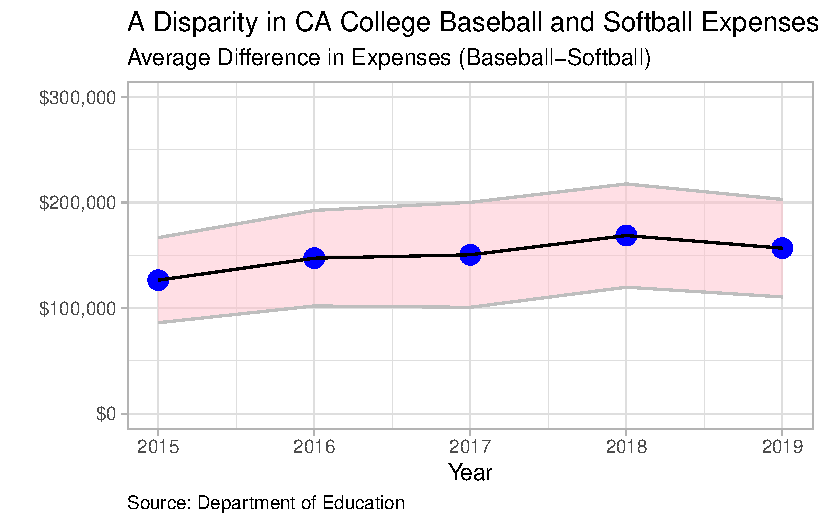
\includegraphics{Report_files/figure-pdf/unnamed-chunk-3-1.pdf}

}

\caption{Above entails an analysis of the differences in average
expenses from 2015 to 2019 for collegiate baseball and softball in
California. The Department of Education collects data yearly on
collegiate sports budgets in accordance to The Equity in Althletics
Disclosure Act. The graph above consists of such data subsetted to
contain soley softball and baseball teams from California in the years
2015 to 2019. The expense for a particular year averaged over all
California softball teams is plotted as a blue triangle, wheras the
expense averaged over all California baseball teams in a particular year
is plotted as a red circle. The highlighted region represents adding or
subtracting one standard error of the average from the plotted averages.
There appears to be more variability in the average expenses for
baseball than for softball in any particular year in California. The
average expenses for baseball are consistantly signifigantly larger than
the expenses for women, although the expenses for both sports tend to
increase at a similiar rate over time.}

\end{figure}%

\begin{Shaded}
\begin{Highlighting}[]
\FunctionTok{library}\NormalTok{(kableExtra)}
\NormalTok{table }\OtherTok{\textless{}{-}}\NormalTok{ sports\_dat }\SpecialCharTok{|\textgreater{}}
  \FunctionTok{group\_by}\NormalTok{(Sport, year) }\SpecialCharTok{|\textgreater{}}
  \FunctionTok{filter}\NormalTok{(total\_exp\_menwomen }\SpecialCharTok{!=} \DecValTok{0}\NormalTok{) }\SpecialCharTok{|\textgreater{}}
  \FunctionTok{summarise}\NormalTok{(}\AttributeTok{mean\_exp =} \FunctionTok{mean}\NormalTok{(total\_exp\_menwomen)) }\SpecialCharTok{|\textgreater{}}
  \FunctionTok{pivot\_wider}\NormalTok{(}\AttributeTok{id\_cols =}\NormalTok{ year, }\AttributeTok{names\_from =}\NormalTok{ Sport, }\AttributeTok{values\_from =}\NormalTok{ mean\_exp) }\SpecialCharTok{|\textgreater{}}
  \FunctionTok{rename}\NormalTok{(}\AttributeTok{Year=}\NormalTok{year, }\AttributeTok{Expenses\_Baseball=}\NormalTok{Baseball, }\AttributeTok{Expenses\_Softball=}\NormalTok{Softball)}

\FunctionTok{kable}\NormalTok{(table)}
\end{Highlighting}
\end{Shaded}

\begin{longtable}[]{@{}rrr@{}}
\toprule\noalign{}
Year & Expenses\_Baseball & Expenses\_Softball \\
\midrule\noalign{}
\endhead
\bottomrule\noalign{}
\endlastfoot
2015 & 397818.2 & 250096.5 \\
2016 & 436379.8 & 269675.2 \\
2017 & 460608.8 & 289536.4 \\
2018 & 492032.7 & 307159.0 \\
2019 & 463564.6 & 294723.3 \\
\end{longtable}

\begin{Shaded}
\begin{Highlighting}[]
\FunctionTok{library}\NormalTok{(rstatix)}
\FunctionTok{t\_test}\NormalTok{(sports\_dat, total\_exp\_menwomen}\SpecialCharTok{\textasciitilde{}}\NormalTok{Sport) }
\end{Highlighting}
\end{Shaded}

\begin{verbatim}
# A tibble: 1 x 8
  .y.                group1   group2      n1    n2 statistic    df             p
* <chr>              <chr>    <chr>    <int> <int>     <dbl> <dbl>         <dbl>
1 total_exp_menwomen Baseball Softball   775   693      6.36 1321. 0.00000000027
\end{verbatim}



\end{document}
